%------------------ vorlage.tex ------------------------------------------------
%
% LaTeX-Vorlage zur Erstellung von Projektdokumentationen
% im Fachbereich Informatik der Hochschule Trier
%
% Basis: Vorlage 'svmono' des Springer Verlags
% Bearbeiter: Hermann Schloß, Christian Bettinger
%
%-------------------------------------------------------------------------------


%------------------ Präambel ---------------------------------------------------
\documentclass[envcountsame,envcountchap deutsch]{i-studis}

\usepackage[utf8]{inputenc}

\usepackage[a4paper]{geometry}
\usepackage[english, ngerman]{babel}

\usepackage[pdftex]{graphicx}
\usepackage{epstopdf}

\usepackage{listings}

\usepackage[german, ruled, vlined]{algorithm2e}
\usepackage{amssymb, amsfonts, amstext, amsmath}
\usepackage{array}
\usepackage[skip=10pt]{caption}
\usepackage[usenames, dvipsnames]{color}
\usepackage[pdftex, plainpages=false]{hyperref}
\usepackage{textcomp}
\usepackage{hyperref}
\usepackage{graphicx}
\usepackage{fancyhdr}
\usepackage{algorithmic}

\usepackage{bibgerm}
\bibliographystyle{geralpha}

\usepackage{makeidx}
\usepackage{multicol}
\makeindex

\pagestyle{myheadings}
\setlength{\textheight}{1.1\textheight}
\setlength{\parindent}{0pt}

\lstset{
	language=[Sharp]C,
	basicstyle=\scriptsize\ttfamily,
	commentstyle=\scriptsize\ttfamily\color{Gray},
	identifierstyle=\scriptsize\ttfamily,
	keywordstyle=\scriptsize\ttfamily,
	stringstyle=\scriptsize\ttfamily,
	tabsize=4,
	numbers=left,
	numberstyle=\tiny,
	numberblanklines=false,
	frame=single,
	framesep=3mm,
	framexleftmargin=7mm,
	xleftmargin=10mm,
	linewidth=144mm,
	captionpos=b,
}



%------------------ Manuelle Silbentrennung ------------------------------------
%\hyphenation{Ele-men-tar-ob-jek-te ab-ge-tas-tet Aus-wer-tung House-holder-Matrix Least-Squares-Al-go-ri-th-men}


%------------------ Titelseite -------------------------------------------------
\begin{document}
\begin{titlepage}
	
	\begin{center}
		{\Huge\bfseries Doku} \\
		{\Huge\bfseries für Thorned King} \\
		
	\end{center}
	
	\begin{figure}[h]
		\centering
		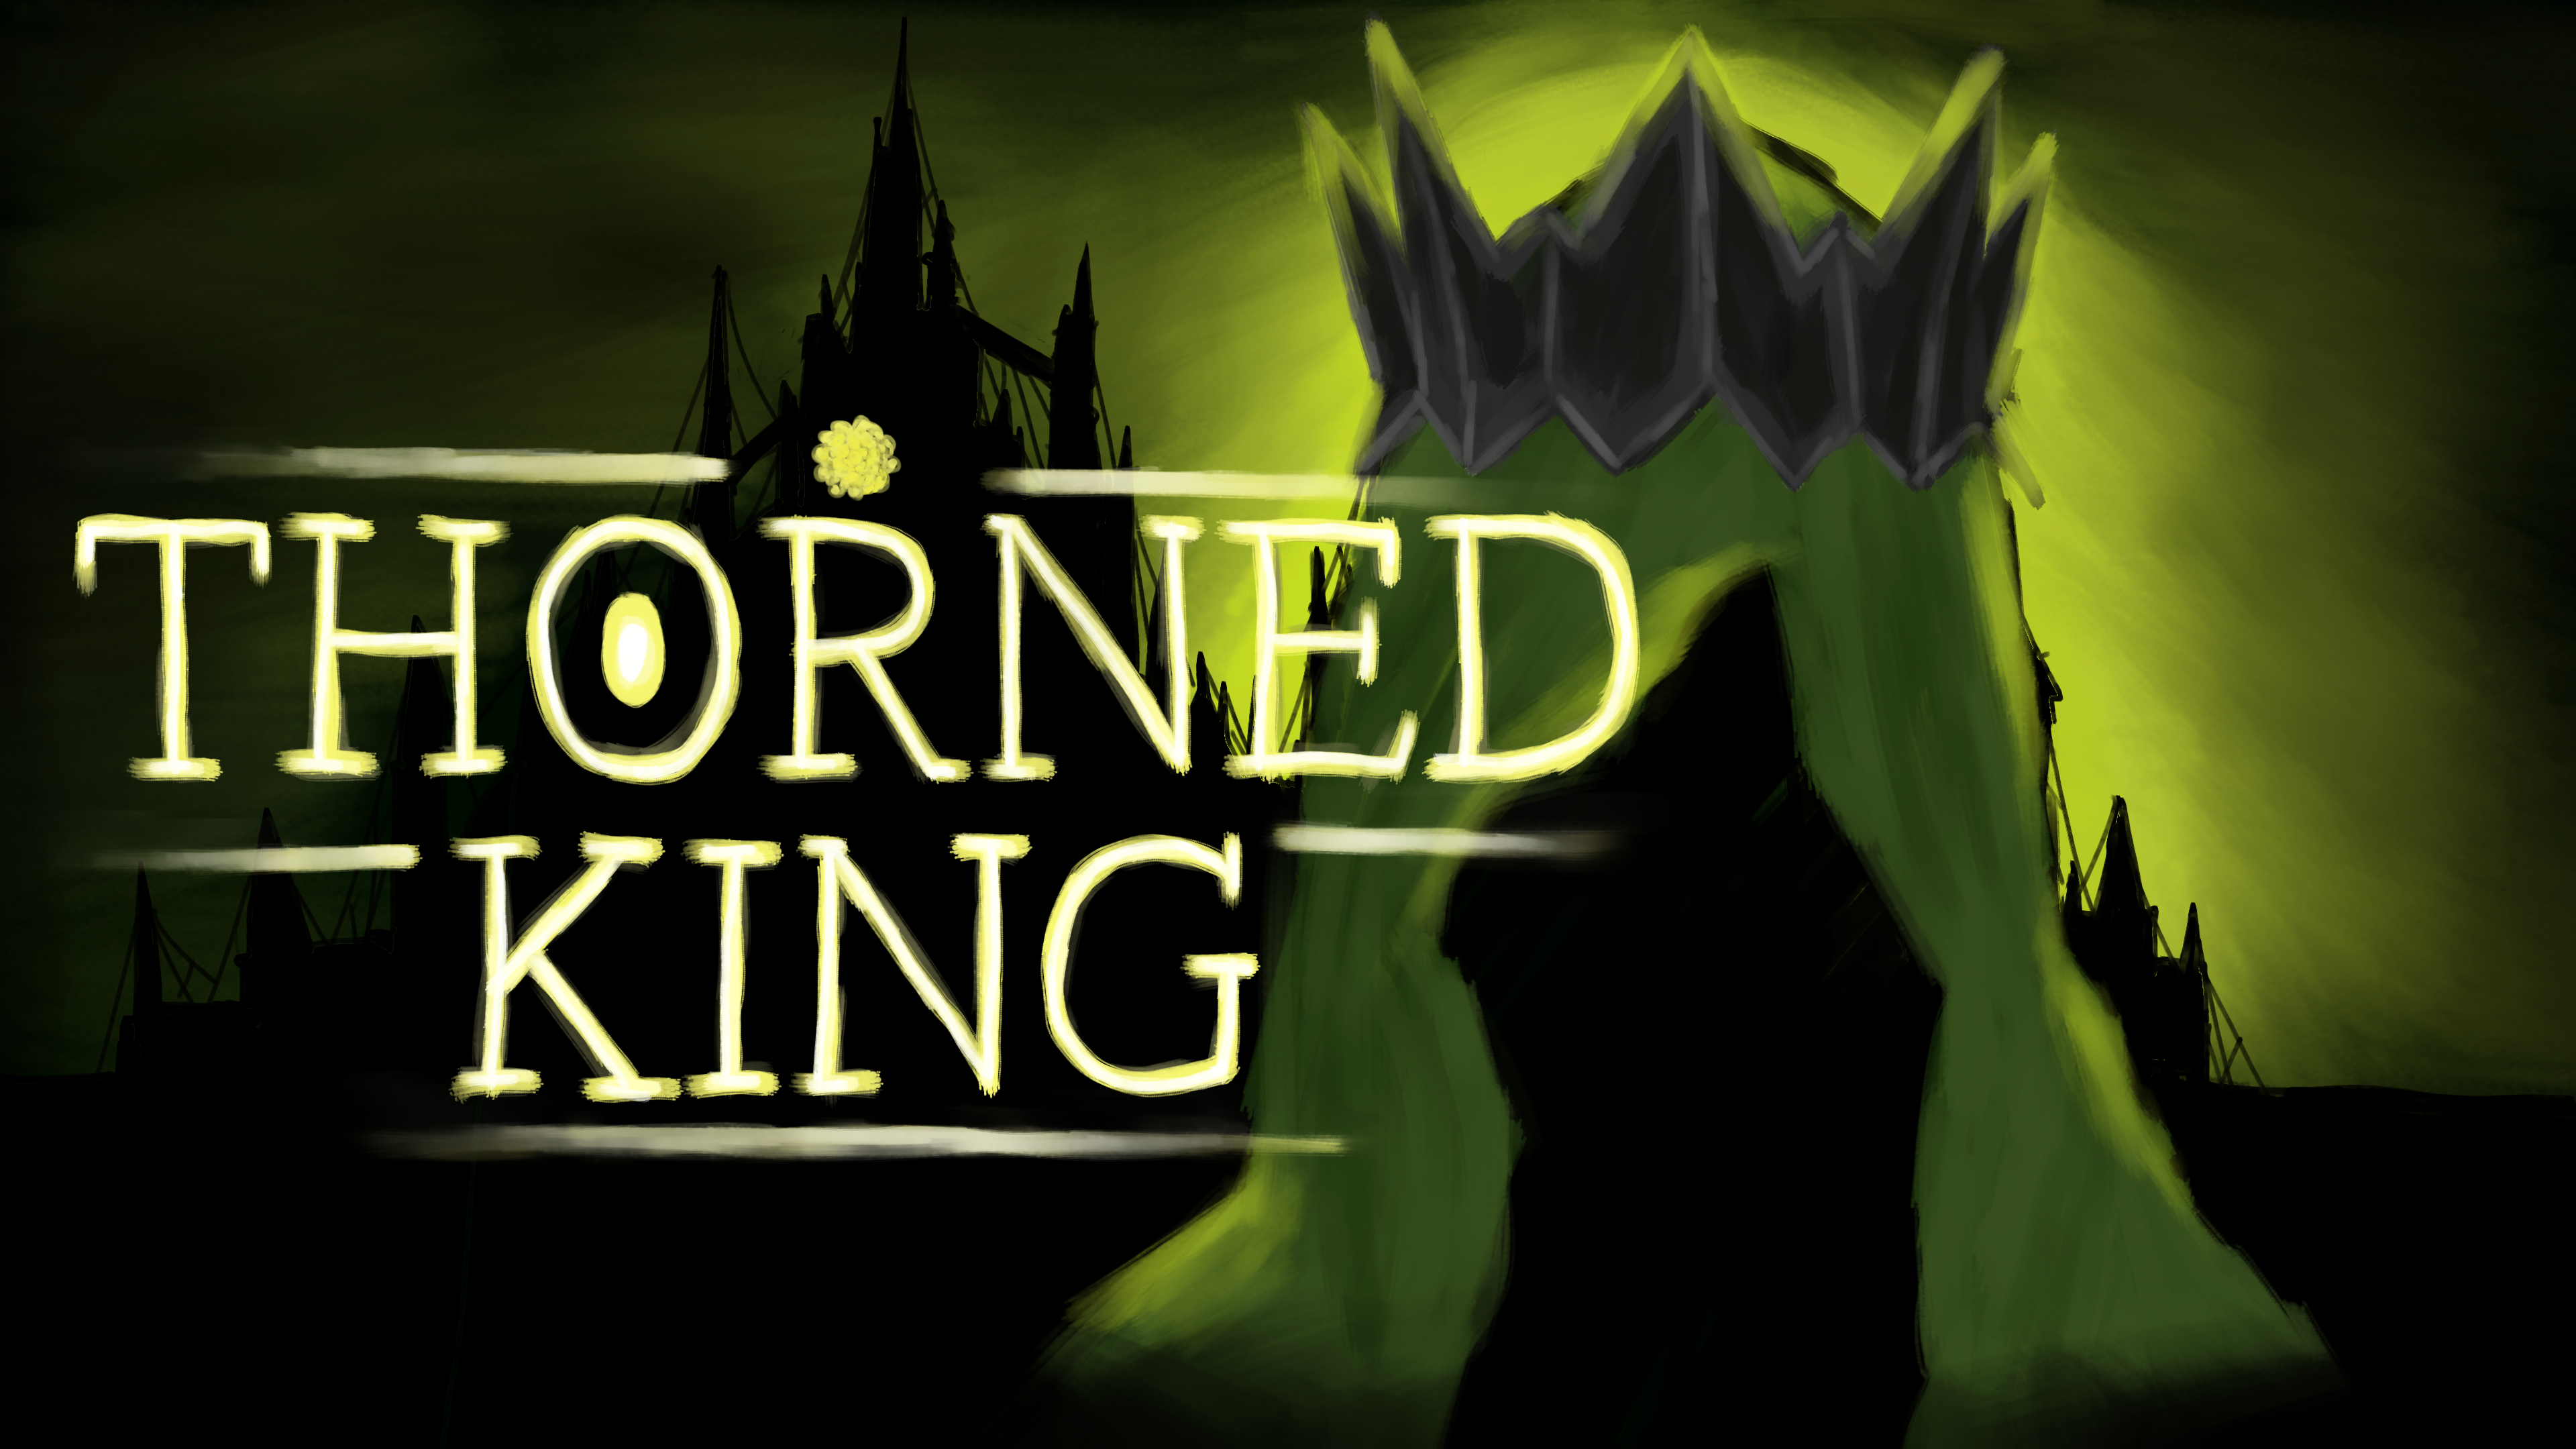
\includegraphics[width=1\textwidth]{images/Krita_ThornedKing.png}
		\label{fig:meinbild}
	\end{figure}
	
	\begin{center}
		Version : 0.0.1 
	\end{center}
	
	
\end{titlepage}
\pagenumbering{arabic}
%------------------ Vorwort, Kurzfassung, Verzeichnisse ------------------------

%\kurzfassung
%Eine Kurzfassung

\tableofcontents										% Inhaltsverzeichnis
%\listoffigures
%\lstlistoflistings

% Du musst nicht alles beschreiben aber du kannst :) Neues Game yey
%------------------ Kapitel ----------------------------------------------------
\chapter{Story}



\section{Weltkarte}
	
	
\begin{figure}[h]
	\centering
	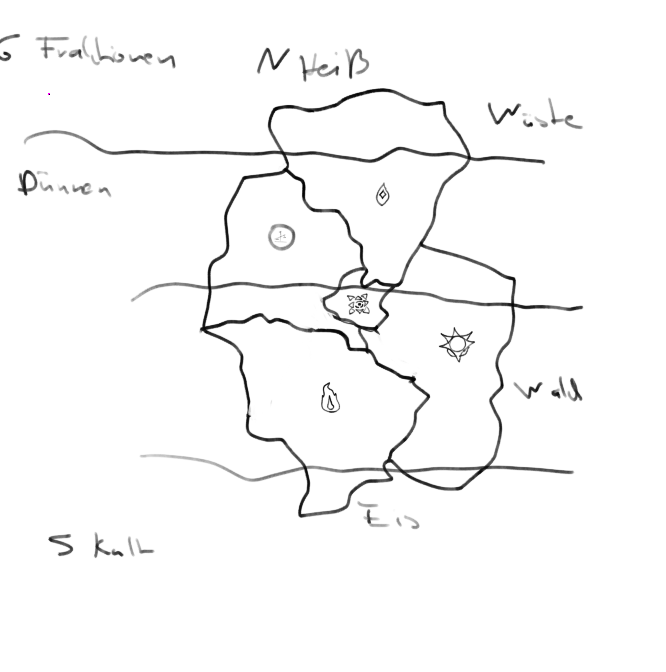
\includegraphics[width=0.7\textwidth]{images/Design/Weltkarte.png}
	\label{fig:meinbild}
\end{figure}
\pagebreak

\section{Randa}
\begin{figure}[h]
	\centering
	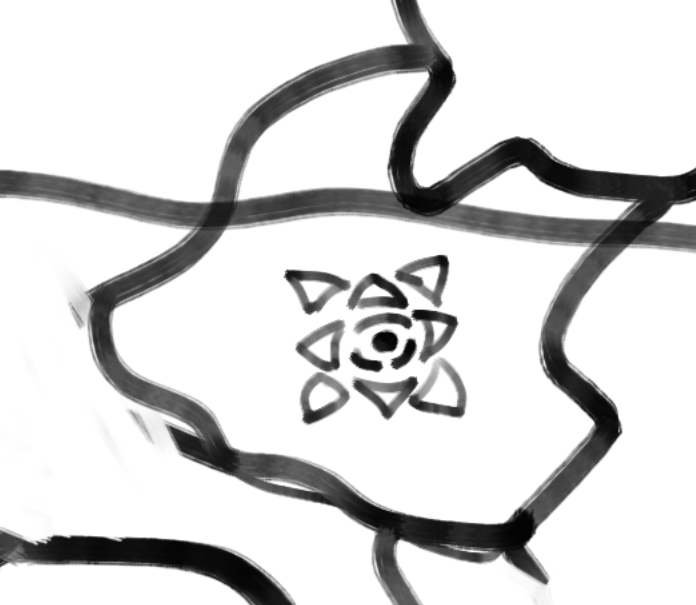
\includegraphics[width=0.2\textwidth]{images/Design/Icon_1.png}
	\label{fig:meinbild}
\end{figure}


Randa ist das Land indem Thorned King spielt.
300 Jahre vor dem Gedornten König war es ein ruhiges Land und wurde von einer Adelsfamilie regiert.
Diese hat durch ihre Handelsbeziehungen mit anderen viele Ressourcen gehabt und konnte somit die Bildung in diesem Land voran treiben. Aus allen regionen der Welt kamen Leute um dort zu studieren.
Die Königsfamilie wurde gepriesen und geliebt.
100 Jahre vor dem gedornten König brachen Kriege um Ressourcen und Terretorien aus. Dabei war Randa Austragungsplatz Nummer 1. Das Königreich hat sich versucht zu wehren aber es wurde geplündert und in schlachten geschlagen. Dies Verwandelte das Land von einer Blumenwiese in ein Niemansland.
Der damaliege Prinz hat verzweifelt nach einer Lösung für Frieden gesucht die seine Vorfahren nicht geschafft haben zu finden. Seine letzte Lösung war es selbst Grund für den Krieg zu sein um alle Königreiche zu vereinen. Somit ging er einen Pakt mit einem Wesen ein welchen ihn zum Teil übernahm.

Danach entstanden überall Dornenranken im Land welche sich immer weiter ausbreiten was die Länder dazu zwingt sich gegen den Gedornten König zu verbünden. Aber keine Expedition dahin war je Erfolgreich weil selbst wenn der König fällt der Schlächter zum neuen König wird. Es muss immer einen König geben wenn es Frieden geben soll.
 

\section{Hamandra}
\begin{figure}[h]
	\centering
	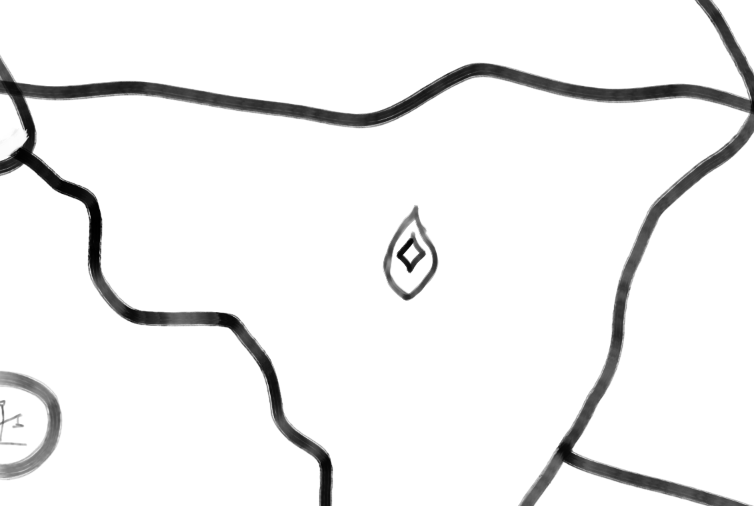
\includegraphics[width=0.2\textwidth]{images/Design/Icon_2.png}
	\label{fig:meinbild}
\end{figure}

Hamandra liegt im Süden  und ist ein von einer Wüste überzogenes Land. Die meisten Menschen leben entlang von Flüssen. Es werden Expeditionen in die Wüste unternommen um Trümmer eines Meterioden zu finden. Diese sind wertvoller Gold und können genutzt werden um Zaubersprüche zu zaubern.
Spliter werden in die Stirn eingesetzt in einem Ritual um ein Magier zu werden. Dies erhalten nur wichtige Menschen und gelerte. Sie können wieder entnommen werden. Wenn jemand lebt stirbt dieser Direkt. Staub wird genutzt um Spruchrollen anzufertigen.

Die Splitter werden als Körper der Gottheit Lanir gesehen welche diese in einem Kampf gegen einen anderen Gott verloren hat.


\section{Silva}
\begin{figure}[h]
	\centering
	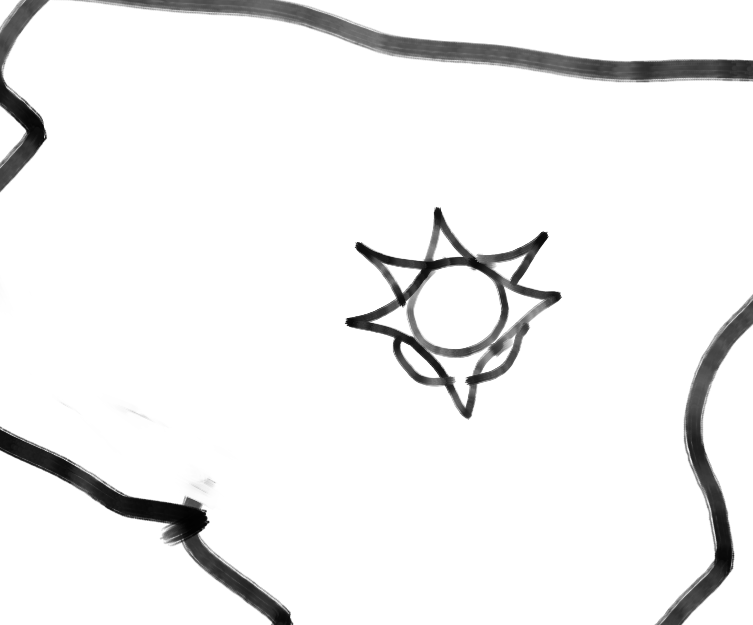
\includegraphics[width=0.2\textwidth]{images/Design/Icon_3.png}
	\label{fig:meinbild}
\end{figure}

Silva ist ein von Wäldern und Pilzen überzogenes Land. Die Menschen die dort leben ernähren sich nur von Pflanzen und Pilzen. Sie beten einen Gott mit dem namen Fangu an. Dieser gibt Leben und nimmt Leben.
Wenn sie sterben wird ein Pilz auf ihren Leichen verteilt. Der Dort Wachsende wird dann von allen Gegessen.


\section{Fraktion 4}
\begin{figure}[h]
	\centering
	
\includegraphics[width=0.2\textwidth]{images/Design/Icon_4.png}
	\label{fig:meinbild}
\end{figure}

\section{}
\begin{figure}[h]
	\centering
	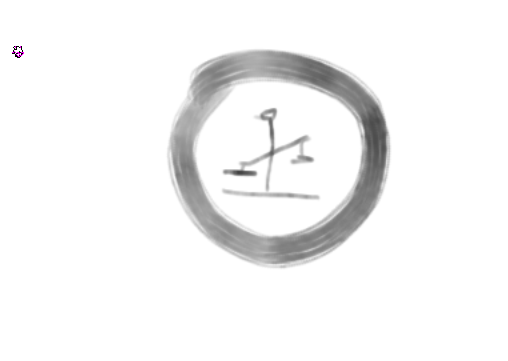
\includegraphics[width=0.2\textwidth]{images/Design/Icon_5.png}
	\label{fig:meinbild}
\end{figure}

\section{Neu Weltler}



\chapter{Game Design}
\section{Spielgebiete}


\subsection{Der Pass (Tutorial)}
\subsection{Der letzte Pfad (Erweiterte Einführung)}
\subsection{Die Brücke}

\subsection{Stadt}
\subsection{Gildenhalle}
\subsection{Waffenhalle}

\subsection{Schlosshof}

\subsection{Schloss}

\subsection{Bibliothek}
\subsection{Alchemiekeller}

\chapter{Level Design}
Da Regels sind da Regels: \\\\
\begin{itemize}
	\item 1. Ein klares Ziel etablieren
	\item 2. Stelle immer mal wieder neue Mechaniken vor
	\item 3. So wenig leeren Raum wie möglich
	\item 4. Führe den Spieler. Spieler wollen in der Regel nach rechts gehen 
	\item 5. Es ist ok wenn Spieler Inhalte nicht finden oder ignorieren 
	\item 6. Wenn Spieler sich außerhalb des Pfades Umsehen sollten sie belohnt werden 
\end{itemize}

\pagebreak
\section{Tutorial Level}
Das Tutorial Level soll eine Einführung in das Spiel darstellen.Lol
Dabei müssen folgende Mechaniken unbedingt vorgestellt werden.
\begin{itemize}
	\item 1. Bewegung
	\item 2. Springen
	\item 3. Dialog
	\item 4. Ausrüstung finden
	\item 5. Barikade zerstören und Loot zum zerstören
	\item 6. Einfache Gegner killen
	\item 7. Speichern
	\item 8. Ziel implementieren
\end{itemize}

\begin{figure}[h]
	\centering
	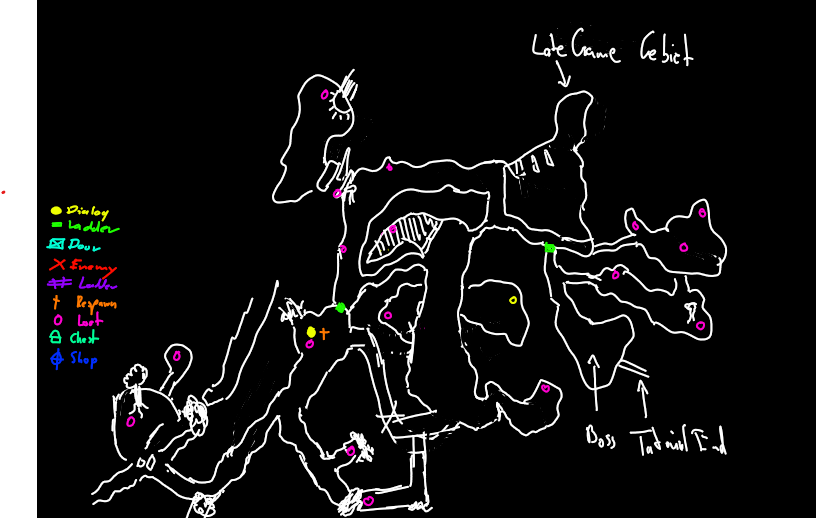
\includegraphics[width=1\textwidth]{images/Design/TutorialLevel_FirstItteration.png}
	\label{fig:meinbild}
\end{figure}

\subsection{}
%------------------ Literaturverzeichnis & Index -------------------------------
%\bibliography{Referenzen}



%------------------ Anhänge ----------------------------------------------------
\begin{appendix}
	%\chapter{Selbstständigkeitserklärung}

\begin{description}

\item[$\Box$] Diese Arbeit habe ich selbstständig verfasst und keine anderen als die angegebenen Quellen und Hilfsmittel verwendet.\\

\item[$\Box$] Diese Arbeit wurde als Gruppenarbeit angefertigt. Meinen Anteil habe ich selbstständig verfasst und keine anderen als die angegebenen Quellen und Hilfsmittel verwendet.\\

Namen der Mitverfasser:
\vspace{3cm}

Meine eigene Leistung ist:
\vspace{3cm}

\end{description}

\vspace{3cm}

\begin{minipage}[t]{3cm}
	\rule{3cm}{0.5pt}
	Datum
\end{minipage}
\hfill
\begin{minipage}[t]{9cm}
	\rule{9cm}{0.5pt}
	Unterschrift der Kandidatin/des Kandidaten
\end{minipage}
	% Selbstständigkeitserklärung
\end{appendix}


\end{document}
